\subsection{Glycan shielding of the AND-gate antigens and the gated surfaceome}
\label{sec:glygen}
A surface antigen can be abundant and tumour-selective yet still hard for a CAR
to engage if its ectodomain is glycan-shielded. We audited glycosylation
evidence for all 205 gene-set genes against GlyGen protein-detail records
(178 genes with a curated record; 27 without one, treated as absence
of evidence rather than evidence of absence). We define a \textbf{shield site}
as a reported N-linked or reported O-linked glycosylation site, excluding
subtype O-GlcNAcylation: O-GlcNAc is an intracellular single-sugar
modification, not a steric shield, and lumping it in would misclassify every
nuclear protein as glycosylated.

\paragraph{Calibration.} The classification was gated before any claim. All
three positive controls carry at least two shield sites (MSLN 4, CD19
3, ERBB2 9), and all four intracellular controls (POLR2A, RPS3,
PCNA, PSMA1) carry reported O-GlcNAc -- proving the subtype field is populated
and the exclusion rule removes real signal. Residual shield-site density in the
intracellular controls (max 0.383 sites/100\,aa, from stray annotations such
as the cell-surface-PCNA literature) sits below the antigen minimum
(0.54/100\,aa). Gate passed 3/3 + 4/4 + ordering.

\paragraph{Gated antigens are more glycosylated, partly by topology
composition.} Within the annotated-surface stratum, 40/54 gated proteins
carry at least one shield site versus 31/61 background (Fisher
$p = 0.013$), and full-length shield density is higher (Mann--Whitney
$p = 6.8e-05$). The topology-composition control tempers the any-site claim:
within single-pass proteins the difference is not significant ($p = 0.171$),
nor within multi-pass ($p = 0.089$) or GPI ($p = 0.491$) strata, so part of
the raw enrichment reflects the gated set's topology mix. The
ectodomain-length-normalized comparison, the biologically relevant measure for
shielding, does survive: gated median 0.88 sites per 100 ectodomain residues
versus background 0.15 ($p = 0.0007$, proteins with annotated ectodomains
$\geq 20$\,aa).

\paragraph{Per-antigen shield table.} The seven AND-gate antigens span two
orders of magnitude of glycan burden (Figure~\ref{fig:glygen}). SLC39A6 is the
heaviest shield in the set -- 22 reported sites backed by 18 distinct
glycan structures -- while PSCA carries none (0 sites over its 114-residue
length), consistent with its small GPI-anchored ectodomain. MSLN's 4
shield sites carry 30 distinct reported structures, matching its known
heavy glycosylation; CLDN6 reports 4 sites on only 220 residues. Among
the approved references, FOLR1's three sites carry 67 structures and
ERBB2 carries 9 sites. Shield burden is thus a per-antigen property that
expression gating does not capture, and it argues for epitope selection away
from reported glycan sites for SLC39A6, MSLN and CLDN6 in particular.

\begin{figure}[t]
\centering
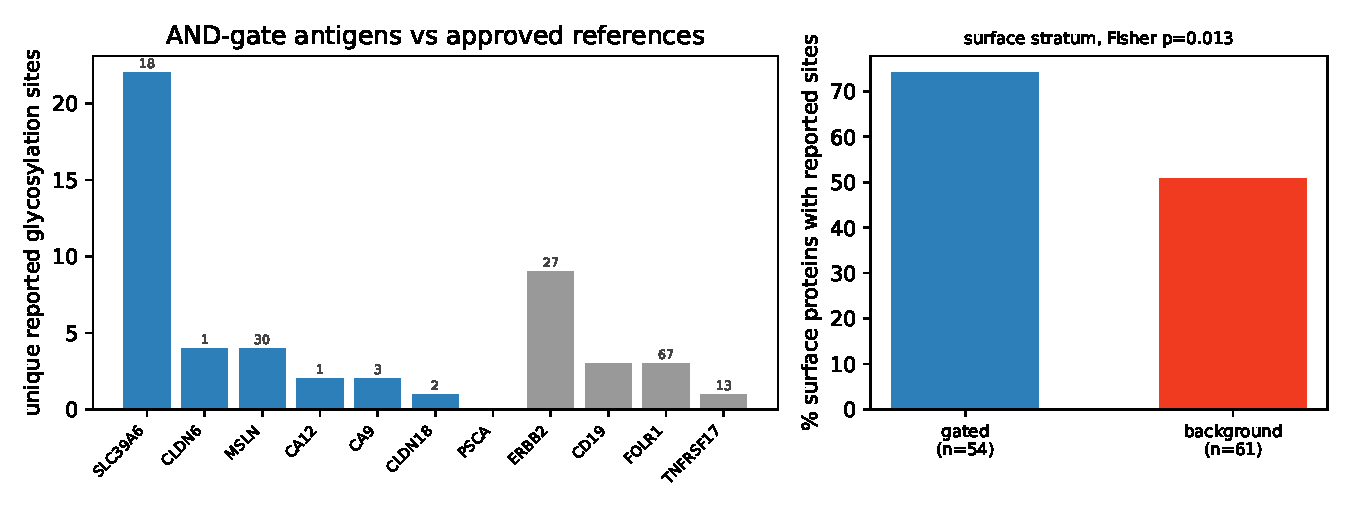
\includegraphics[width=\linewidth]{glygen_fig.pdf}
\caption{Glycan-shield audit. Left: unique reported shield sites for the seven
AND-gate antigens (blue) and four approved CAR-T references (grey); numbers
above bars count distinct GlyTouCan glycan structures. Right: fraction of
annotated-surface proteins carrying at least one shield site, gated versus
background.}
\label{fig:glygen}
\end{figure}
